%% Standalone supplementary material: second implementation (FEniCSx) of blobInTreacle and audit of the interface formulation.
%% DRAFT. Build (from this directory):  latexmk -pdf supplement_fenicsx_blobintreacle.tex
%% It does not read article.aux (no cross-references to the main article), so it builds on its own.
%% Data, scripts and provenance: paper-data/fenicsx_blobintreacle/ (README.md there).
\documentclass[sn-mathphys,Numbered]{sn-jnl}
\usepackage{graphicx}
\usepackage{amsmath,amssymb,amsfonts,bm}
\usepackage{xcolor}
\usepackage{manyfoot}
\usepackage{booktabs}
\usepackage{siunitx}
\usepackage{float}
\usepackage[utf8]{inputenc}
\usepackage[onehalfspacing]{setspace}
\usepackage[section]{placeins}
\usepackage{geometry}
\geometry{a4paper,textwidth=15cm,textheight=24cm}
\setlength{\parskip}{\baselineskip}

%% S-prefixed numbering
\renewcommand{\thesection}{S\arabic{section}}
\renewcommand{\thefigure}{S\arabic{figure}}
\renewcommand{\thetable}{S\arabic{table}}
\renewcommand{\theequation}{S\arabic{equation}}

\newcommand{\todo}[1]{\par\noindent\textcolor{red}{\rule{\linewidth}{0.8pt}}\par\nopagebreak
	\noindent{\small\color{red!70!black}\textbf{AUTHOR NOTE:} #1\par}\nopagebreak
	\noindent\textcolor{red}{\rule{\linewidth}{0.8pt}}\par}
\newcommand{\citetodo}[1]{\textcolor{red}{[\textbf{cite:}~#1]}}
\newcommand{\pending}[1]{\textcolor{red}{[\textbf{PENDING:}~#1]}}

\begin{document}

\title[Supplementary material: FEniCSx blobInTreacle]{Supplementary material: a second implementation of blobInTreacle (FEniCSx) and an audit of the interface formulation}

\author*[1]{\fnm{Philip} \sur{Cardiff}}\email{philip.cardiff@ucd.ie}
\author[1]{\fnm{Sairam} \sur{Pamulaparthi Venkata}}

\affil[1]{\orgdiv{School of Mechanical and Materials Engineering}, \orgname{University College Dublin}, \orgaddress{\country{Ireland}}}


\maketitle

\todo{DRAFT for review (draft pull request, issue \#50). Author list and order are placeholders for the authors to decide. Every number is taken from the run records listed in \texttt{paper-data/fenicsx\_blobintreacle/README.md} and the CSV files there; the wording follows the independent review of the evidence package (findings accepted, claims not supported). Not yet reviewed by a human outside the lineage that produced the evidence (Section~\ref{sec:fx_independence}).}

%%%%%%%%%%%%%%%%%%%%%%%%%%%%%%%%%%%%%%%%%%%%%%%%%%%%%%%%%%%%%%%%%%
\section{Purpose, scope and independence}\label{sec:fx_scope}
%%%%%%%%%%%%%%%%%%%%%%%%%%%%%%%%%%%%%%%%%%%%%%%%%%%%%%%%%%%%%%%%%%
The only reference for blobInTreacle in the verification suite is category C-weak: figure-extracted interface shapes from a preprint~\citep{Liu2013} of~\citet{Liu2014}, on a coarse mesh, with first-order time integration.
Issue \#50 asked for an independent numerical solution with mesh and time-step convergence.
This supplement reports a second implementation of the problem, a monolithic finite element code written with FEniCSx, run on the same quadrilateral mesh topology as the solids4foam tutorial and refined jointly with it, and what it shows about (i) the steady state, (ii) the time integration and (iii) the interface force transfer of the solids4foam tutorial.
It is supplementary material: it adds a cross-code check of the steady state of the original model and a quantified model-form sensitivity; it does not replace the C-weak reference, and it does not settle the temporal accuracy of the suite.

\paragraph{Independence statement.}\label{sec:fx_independence}
What is independent is the numerics: a monolithic Taylor--Hood finite element discretisation with a Newton solver, against a partitioned cell-centred finite volume code with IQN-ILS coupling.
What is not independent: the work was done by the same research group as the solids4foam results, by AI coding agents of the same model family that also acted as the verifiers (the ``verifier'' of the E-AREA experiment of Section~\ref{sec:fx_formulation} is the agent lineage that wrote it), and the problem definition, the mesh topology (480 fluid and 120 solid cells at the first level, the same 24 interface chords), the extraction of the solids4foam reference series and the Richardson/GCI routine are shared.
The solids4foam interface measure was identified by reading its source; the FEniCSx code reproduces that model, so a shared misreading of the problem definition would not be visible in the comparison.
An independent referee-style review by a further agent of the same family was carried out; its accepted findings and the claims it rejected define the wording below.
No review by a human outside this lineage has yet taken place.
The result is therefore a second implementation by the same group, not an independent verification by a different group, and the original request of issue \#50 for a different code (FEBio) is not met by it.

%%%%%%%%%%%%%%%%%%%%%%%%%%%%%%%%%%%%%%%%%%%%%%%%%%%%%%%%%%%%%%%%%%
\section{Solver and exact original model}\label{sec:fx_solver}
%%%%%%%%%%%%%%%%%%%%%%%%%%%%%%%%%%%%%%%%%%%%%%%%%%%%%%%%%%%%%%%%%%
\paragraph{Solver.}
DOLFINx 0.10.0 (PETSc 3.25.6, MUMPS 5.8.2, MPICH 5.0.1) with a monolithic formulation on one mesh covering the fluid and the solid.
The unknowns are a velocity $\bm u$ (continuous $Q_2$, continuous across the interface, which imposes no-slip and the kinematic condition exactly in the discrete problem), a pressure $p$ ($Q_1$, constrained to zero strictly inside the solid) and a displacement $\bm d$ ($Q_2$, the solid displacement, and a harmonic extension in the fluid that moves the mesh).
The fluid is the incompressible Navier--Stokes system in an arbitrary Lagrangian--Eulerian form on the reference configuration, Galerkin, without stabilisation ($Re=O(1)$); the solid is linear elastic with linear geometry; the traction balance on the interface is the natural condition obtained by adding the two momentum residuals with a shared test function.
The nonlinear system is solved by PETSc SNES (Newton, line search, relative tolerance $10^{-9}$, absolute $10^{-10}$).
Production runs use backward Euler ($\theta=1$) for the steady-state studies and backward differentiation (BDF2 with a backward Euler first step) for the transient studies.
The quadrilateral meshes are the tutorial's blocking refined by factors $F=0.5$, $1$, $2$, $4$ (150, 600, 2400, 9600 cells in total; interface 12, 24, 48, 96 chords) and are generated and hash-checked (Table~\ref{tab:fx_meshes}).

\begin{table}[htbp]
\centering
\caption{Meshes of the FEniCSx studies (quadrilateral, straight interface chords as in the solids4foam tutorial). The solids4foam levels x0.5 to x4 have the same cell counts.}\label{tab:fx_meshes}
\begin{tabular}{@{}lrrl@{}}
\toprule
Level & Cells (fluid/solid) & Interface chords & sha256 of the mesh file (prefix) \\
\midrule
$F=0.5$ & 120/30 & 12 & 39eebdbb \\
$F=1$ & 480/120 & 24 & 2c8ce4d9 \\
$F=2$ & 1920/480 & 48 & 599a81e6 \\
$F=4$ & 7680/1920 & 96 & 50e9ac2d \\
\bottomrule
\end{tabular}
\end{table}

\paragraph{The original model.}
The case is that of the solids4foam tutorial \texttt{blobInTreacle}: channel $[0,6.5]\times[-0.5,1]\,\mathrm{m}$, half-cylinder of radius $0.5\,\mathrm{m}$ centred at $(1.5,-0.5)\,\mathrm{m}$ with a fixed base, plane strain; fluid $\rho_f=1$, $\nu_f=1$; solid $\rho_s=1$, $\lambda=500\,\mathrm{Pa}$, $\mu=50\,\mathrm{Pa}$; inlet $u_x=g(t)(1+2y)(1-y)$ with $g=\tfrac12[1-\cos(\pi t/2)]$ for $t\le2$ and $1$ afterwards; no-slip walls and interface; $p=0$ at the outlet.
The solid in the tutorial (and in the preprint) is \emph{linear-geometry} linear elastic, small strain on the undeformed mesh, although the apex moves $0.12\,\mathrm{m}$ on a radius of $0.5\,\mathrm{m}$.
The FEniCSx code uses the same solid.
(A finite-strain St~Venant--Kirchhoff solid is a different model: with solids4foam it is $30\%$ larger in $u_x(t=1)$ and the full-amplitude coupled problem did not reach a steady state in any code tried, as reported on issue \#50; the suite's inventory entry ``large (TL, StVK)'' for this case therefore does not describe the original model.)
Other differences from the solids4foam tutorial are the fluid discretisation (Galerkin $Q_2/Q_1$ against cell-centred finite volume with linear-upwind convection), the mesh motion (harmonic extension with a $1/\mathrm{cell\ volume}$ stiffness against a velocity Laplacian), the solid discretisation ($Q_2$ against a cell-centred scheme), the outlet (natural gradient-form condition against $p=0$ with zero-gradient velocity) and the coupling (monolithic against partitioned); their effect was not isolated.

%%%%%%%%%%%%%%%%%%%%%%%%%%%%%%%%%%%%%%%%%%%%%%%%%%%%%%%%%%%%%%%%%%
\section{Two interface formulations: M2 and M1}\label{sec:fx_formulation}
%%%%%%%%%%%%%%%%%%%%%%%%%%%%%%%%%%%%%%%%%%%%%%%%%%%%%%%%%%%%%%%%%%
Let $\bm\sigma_f$ be the fluid stress, $\bm n_\mathrm{cur}$ the unit normal of the current interface, $\bm a=J\bm F^{-T}\bm N$ the Nanson vector of a reference interface element ($J_s=|\bm a|=\mathrm{d}s/\mathrm{d}S_0$ the interface stretch).
The force the fluid exerts on a reference element is $\bm\sigma_f\bm a\,\mathrm{d}S_0$.
\begin{description}
\item[M1] (exact force balance) The solid receives $\bm\sigma_f\bm a=J_s\bm\sigma_f\bm n_\mathrm{cur}$ per reference area, i.e.\ equal and opposite forces on corresponding interface patches.
It is the condition stated in the preprint (the balance of $\int_{\phi(e,t)}\bm\sigma_f\bm n_f\,\mathrm{d}a$ and $\int_e\bm\sigma_s\bm n_s\,\mathrm{d}A$ on every part $e$ of the interface), and in the monolithic code it needs no extra term.
\item[M2] (solids4foam tutorial) The solid receives $\bm\sigma_f\bm n_\mathrm{cur}$, the traction per \emph{current} area, applied per \emph{reference} area.
By source inspection of solids4foam (\texttt{fluidSolidInterface}: face-to-face copy of the fluid traction, no area weighting; \texttt{solidTraction} on the undeformed solid mesh) this is what the tutorial does; in the FEniCSx code it is the M1 residual plus the term $\int(1-1/J_s)\bm\sigma_f\bm a\cdot\bm\varphi\,\mathrm{d}S_0$.
\end{description}
The two differ by $(1-J_s)\bm\sigma_f\bm n_\mathrm{cur}$.
With the interface stretch ranging over $0.89$--$1.28$ around the blob, M2 does not deliver to the solid the force the fluid exerts, and is not power-conjugate with the no-slip kinematics at finite motion.
This is a statement about a modelling choice in a linear-geometry benchmark, established at the level of the formulation (algebra, checked on random deformation gradients) and of the discrete evidence in this supplement (evidence levels~1 and~2 only); no level-3 claim is made, no claim that the solids4foam coupling is defective, and no claim that either measure is the correct continuum model: both are applied to a small-strain solid at $24\%$ apex strain, so M1 is exact only in the force balance, not in the solid kinematics.
\emph{The original benchmark is therefore not one model}: the tutorial (reference A) is M2, the preprint (reference B) states the M1 balance, and the two give steady apex displacements that differ by far more than any discretisation error (Section~\ref{sec:fx_steady}).
Both are reported here and never combined.

\paragraph{Same-lineage diagnostic (E-AREA).}
To test on the solids4foam side whether the M2/M1 difference is the cause of the offset to the preprint, a user-library boundary condition scales the transferred traction by the ratio of current to reference face area (so that the force applied to the solid equals the force the fluid exerts), with solids4foam itself unmodified (binary checksums unchanged).
It was written, run and checked by the same agent lineage and is a diagnostic of the sensitivity, not a verification of the coupling: that the applied and fluid-reported forces agree to $10^{-6}$ holds by construction of the face-wise scaling; its one non-tautological check (the base reaction against the fluid-reported force) is \emph{not} met in $x$ ($0.974$ at x1 and $0.986$ at x2 against a preregistered $1.00\pm0.01$), and the stress estimator used for the reaction is itself $1.8$--$2.5\%$ in error on the interface patch where the true force is known.
Only three levels (x0.5, x1, x2) exist; the x4 level was not run.
Its ratios to the original are in Table~\ref{tab:fx_fourway}.

%%%%%%%%%%%%%%%%%%%%%%%%%%%%%%%%%%%%%%%%%%%%%%%%%%%%%%%%%%%%%%%%%%
\section{Steady state: spatial convergence of M2 and M1}\label{sec:fx_steady}
%%%%%%%%%%%%%%%%%%%%%%%%%%%%%%%%%%%%%%%%%%%%%%%%%%%%%%%%%%%%%%%%%%
Both sequences use four levels, $h=N_\mathrm{cells}^{-1/2}$, the finest three for the order and the Richardson limit, and the rules of the main article (monotone, $0.5\le p\le3$, $F_s=1.25$); the coarsest three levels give the same limits within the coarsest-triple GCI.
All runs reached the registered steady criterion (apex drift below $10^{-8}$ relative), converged in every Newton step (with a few step-norm acceptances in transients, none at steady state), and the steady states are independent of the time step and of the scheme: the M2 apex at $F=0.5$, $1$, $2$ with $\Delta t=0.04$ equals the $\Delta t=0.01$ value in all eight printed digits, M1 steady values at $\Delta t=0.04$, $0.02$, $0.01$ ($F=1$) agree to $\le1.6\times10^{-10}$ and at $F=2$, $4$ ($\Delta t=0.04$ against $0.02$) to $\le2\times10^{-9}$, and M1 with Crank--Nicolson agrees to $6\times10^{-8}$.
Disclosures: the M2 sequence mixes $\Delta t=0.01$ ($F\le2$, $t_\mathrm{end}=10$, commit c8a4b0a) and $\Delta t=0.04$ ($F=4$, $t_\mathrm{end}=6$, commit 1484d94); the minimum Jacobian of the fluid mesh falls monotonically with refinement ($0.766$, $0.742$, $0.685$, $0.610$ for M2; $0.557$ at $F=4$ for M1) and $F=8$ was not run; the meshes have straight chords (solid area error $-0.285\%$ at $F=1$, $-0.018\%$ at $F=4$), and a curved geometry changes the apex by up to $0.15\%$ at $F=1$, which exceeds the GCI of $u_x$ and is not included in it.

\begin{table}[htbp]
\centering
\caption{Steady apex displacement and forces, FEniCSx, finest three levels ($F=1,2,4$; $h=N^{-1/2}$). $F_x$, $F_y$ are the exact interface integrals of the fluid force (for M1 the force applied to the solid). Source: \texttt{data/steady\_convergence.csv}.}\label{tab:fx_steady}
\begin{tabular}{@{}llrrr@{}}
\toprule
Model & Quantity & $p$ & Richardson limit & GCI (\%) \\
\midrule
M2 & $u_x$ (m) & 1.41 & 0.120286 & 0.048 \\
M2 & $u_y$ (m) & 1.94 & $-0.0139255$ & 0.016 \\
M2 & $F_x$ (N/m) & 2.03 & 16.2607 & 0.017 \\
M2 & $F_y$ (N/m) & 1.82 & $-25.5472$ & 0.008 \\
M2 & $F_y$, weak form & 0.94 & $-25.5415$ & 0.52 \\
M2 & pressure drop (Pa) & 1.94 & 35.9961 & 0.008 \\
M1 & $u_x$ (m) & 1.52 & 0.129372 & 0.032 \\
M1 & $u_y$ (m) & 1.46 & $-0.0117001$ & 0.060 \\
M1 & $F_x$ (N/m) & 2.06 & 16.3184 & 0.016 \\
M1 & $F_y$ (N/m) & 1.90 & $-25.7257$ & 0.006 \\
M1 & $F_y$, weak form & 0.94 & $-25.7196$ & 0.52 \\
M1 & pressure drop (Pa) & 1.97 & 36.0482 & 0.008 \\
\bottomrule
\end{tabular}
\end{table}

The apex displacements converge at observed orders between 1.4 and 1.9 and the weak-form $F_y$ at 0.9, not at the nominal two.
The low order of $F_y$ comes from its viscous part ($p=0.69$; a small difference of large terms that includes the corner nodes where the base meets the interface) while the pressure part converges at 1.97, and the order of $u_x$ is likely affected by the floor--interface corner singularity; this is asserted, not tested.
The GCI values are therefore estimates of the discretisation error with $p<2$, to be quoted with the order, and are not a bound.

\begin{figure}[htbp]
\centering
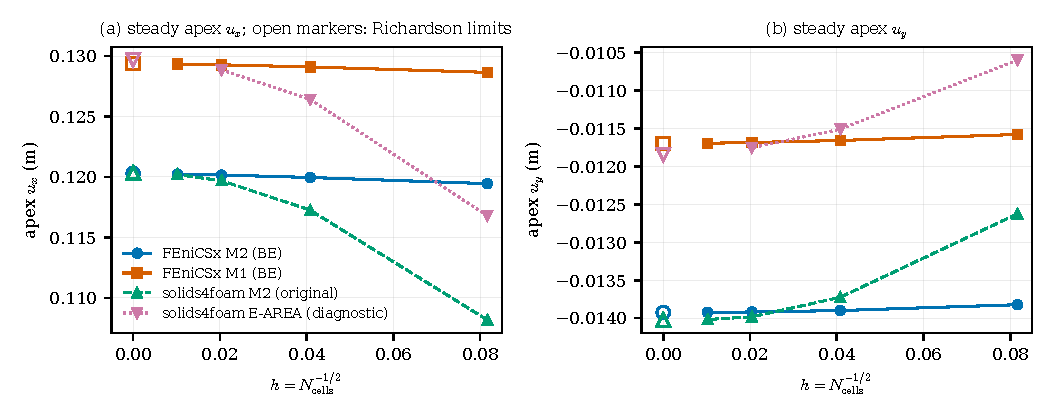
\includegraphics[width=\textwidth]{paper-data/fenicsx_blobintreacle/figures/fenicsx_blob_spatial}
\caption{blobInTreacle, steady apex displacement against $h=N_\mathrm{cells}^{-1/2}$: FEniCSx M2 and M1 (backward Euler), solids4foam M2 (the tutorial, regenerated series) and the E-AREA diagnostic. Open markers at $h=0$ are the Richardson limits (finest three levels; E-AREA: its three levels). Source: \texttt{paper-data/fenicsx\_blobintreacle/data/steady\_levels.csv}.}\label{fig:fx_spatial}
\end{figure}

\paragraph{Model-form difference.}
At every level and in the limits, M1 against M2 gives $u_x$ larger by $7.5\%$ ($u_x^{M1}/u_x^{M2}=1.0755$ in the limits) and $|u_y|$ smaller by $16\%$ ($u_y^{M1}/u_y^{M2}=0.840$), stable under refinement to $<0.15$ percentage points, while the fluid-reported $F_x$ differs by $0.36\%$ and the pressure drop by $0.15\%$; the base reaction in $x$ differs by $13\%$.
The difference sits in the force the solid actually receives, not in the fluid solution, and it exceeds either sequence's GCI by more than an order of magnitude.

%%%%%%%%%%%%%%%%%%%%%%%%%%%%%%%%%%%%%%%%%%%%%%%%%%%%%%%%%%%%%%%%%%
\section{Cross-code comparison of the steady state}\label{sec:fx_crosscode}
%%%%%%%%%%%%%%%%%%%%%%%%%%%%%%%%%%%%%%%%%%%%%%%%%%%%%%%%%%%%%%%%%%
The solids4foam series was regenerated for this comparison (commit 1576edcc4, OpenFOAM v2512, \texttt{couplingReuse 5}, amplitude 1, levels x0.5 to x4, analysed at $t=4$; x1 from the $t=10$ tutorial run, x4 with $\Delta t=0.005$) and differs from the numbers shipped with the tutorial by $2\times10^{-5}$ to $5\times10^{-4}$ in absolute apex displacement.
Its inlet flux exceeds the analytic value by $0.54\%$ at x1 and $0.03\%$ at x4; a linearised correction does not change the comparison at the level quoted.
FEniCSx M2 and solids4foam M2 (the same model) compare as in Table~\ref{tab:fx_crosscode}.

\begin{table}[htbp]
\centering
\caption{Steady state, FEniCSx M2 against solids4foam M2: relative difference at equal cell counts and between the Richardson limits (finest three levels), with the GCI of each. Source: \texttt{data/steady\_crosscode.csv}.}\label{tab:fx_crosscode}
\begin{tabular}{@{}lrrrrr@{}}
\toprule
Quantity & x1/F1 (\%) & x2/F2 (\%) & x4/F4 (\%) & limits (\%) & GCI s4f / FEniCSx (\%) \\
\midrule
$u_x$ & $+2.30$ & $+0.40$ & $+0.03$ & $-0.05$ & 0.15 / 0.05 \\
$u_y$ & $+1.28$ & $-0.46$ & $-0.67$ & $-0.70$ & 0.05 / 0.02 \\
$F_x$ & $+2.50$ & $+0.34$ & $-0.08$ & $-0.18$ & 0.14 / 0.02 \\
$F_y$ & $+2.19$ & $+0.42$ & $+0.02$ & $-0.10$ & 0.16 / 0.01 \\
Pressure drop & $+2.85$ & $+0.70$ & $+0.10$ & $-0.14$ & 0.31 / 0.01 \\
\bottomrule
\end{tabular}
\end{table}

The steady apex $u_x$, the interface force and the pressure drop agree within $0.2\%$ between two discretisation families (monolithic finite element, partitioned finite volume), which is not what a common numerical defect would give.
At the first level the two differ by $2.3\%$ in $u_x$, which is mostly the coarse-mesh error of the solids4foam tutorial mesh against its own limit ($-2.5\%$).
Apex $u_y$ agrees to $0.7\%$ only, and this is \emph{not} resolved below about $1\%$: $u_y$ amplifies differences in the interface load by a factor of about six for the load resultant ($0.70\%$ in $u_y$ for a $0.12\%$ difference in $F_x$) and about ten per $15^\circ$ bin of the load distribution ($0.06\%$ in $F_x$, $0.036\%$ in $F_y$, at most $0.012\,\mathrm{N}$ per bin giving $0.62\%$), a property of the solid established by replacing only the load in a solid-only calculation.
Those amplification factors are a sensitivity estimate.
The load difference that has to be amplified is itself not bounded independently of the discrepancy it is meant to explain.
The preregistered same-shape test of the fluid load on the solids4foam deformed shape (agreement if the resultants agree to $0.13\%$ and every $15^\circ$ bin to $0.02\,\mathrm{N}$) returned DISAGREE against the coupled solids4foam load (resultant $F_x$ $-0.134\%$, marginal by $0.004\%$; bins and $F_y$ pass); against the load of a static-wall solids4foam fluid calculation on the same shape (chosen after the first comparison, $F_x$ $-0.078\%$) it passes, and that difference alone reproduces about $92\%$ of the $u_y$ residual.
The solids4foam coupled fluid state is not the static-wall fixed point ($F_x$ $0.056\%$), for reasons not tested.
The two results are reported side by side; the second does not replace the first.
We therefore state only that $u_y$ agrees to $0.7\%$ and that a $u_y$ uncertainty of order $1$--$2\%$ is appropriate for either code, not that it agrees within a propagated uncertainty.
Table~\ref{tab:fx_fourway} places both codes and both interface measures together.

\begin{table}[htbp]
\centering
\caption{Four-way steady table: apex displacement (m), interface force (N/m, exact interface integral; solids4foam: the forces function object) and base reaction $R_x$, finest level and Richardson limit. The E-AREA limit uses its three levels (x0.5, x1, x2) and overshoots by about $0.2\%$ when the same triple is applied to the original series; it is a same-lineage diagnostic, not a verified solution. Source: \texttt{data/fourway\_M1\_M2.csv}.}\label{tab:fx_fourway}
\small
\begin{tabular}{@{}lrrrrr@{}}
\toprule
 & s4f M2 & FEniCSx M2 & s4f E-AREA & FEniCSx M1 \\
\midrule
$u_x$ finest & 0.120208 (x4) & 0.120240 (F4) & 0.128852 (x2) & 0.129339 (F4) \\
$u_x$ limit & 0.120349 & 0.120286 & 0.129675 & 0.129372 \\
$u_y$ finest & $-0.014018$ & $-0.013924$ & $-0.011754$ & $-0.011695$ \\
$u_y$ limit & $-0.014023$ & $-0.013925$ & $-0.011844$ & $-0.011700$ \\
$F_x$ limit & 16.290 & 16.261 & 16.389 & 16.318 \\
$R_x$ limit & $-14.200$ & $-14.206$ & $-16.288$ & $-16.307$ \\
\bottomrule
\end{tabular}
\end{table}

The E-AREA to M2 ratios in the limits ($u_x$ $1.0755$, $u_y$ $0.842$) match the FEniCSx M1 to M2 ratios ($1.0755$, $0.840$) to $0.03\%$ and $0.2\%$, which is consistent with the interface measure being the cause of the difference between the two formulations on the solids4foam side.
The E-AREA $u_y$ limit ($-0.011844$) differs from the FEniCSx M1 limit by $1.2\%$ (GCI $0.96\%$ for E-AREA), and no agreement is claimed for it.
The M1 limits ($u_x=0.12937$) are consistent with the value read off the preprint's coarse-mesh figure ($0.1297$); that value comes from a digitised figure of a coarse mesh, the journal article was not accessed, and no agreement with the preprint, and no statement of which model is correct, is made.

%%%%%%%%%%%%%%%%%%%%%%%%%%%%%%%%%%%%%%%%%%%%%%%%%%%%%%%%%%%%%%%%%%
\section{Temporal verification and its limits}\label{sec:fx_time}
%%%%%%%%%%%%%%%%%%%%%%%%%%%%%%%%%%%%%%%%%%%%%%%%%%%%%%%%%%%%%%%%%%
\paragraph{What was done.}
M2, $F=1$ (600 cells; itself not spatially converged), $t=1$ (still within the inlet ramp), $\Delta t=0.04$ to $0.0025$, backward Euler, BDF2 and (consistent) Crank--Nicolson, against a BDF2 run of the same scheme at $\Delta t=0.0025$ and, for the second-order claim, an independent finer BDF2 run at $\Delta t=0.00125$.
Table~\ref{tab:fx_time} and Figure~\ref{fig:fx_temporal} give the result.

\begin{table}[htbp]
\centering
\caption{Temporal behaviour at $t=1$ (M2, $F=1$). $p$ from \texttt{convergence.analyse} on the finest three levels, or ``--'' when the sequence is not accepted. Pairwise orders against the $\Delta t=0.0025$ BDF2 reference. Source: \texttt{data/time\_orders\_t1\_F1\_M2.csv}.}\label{tab:fx_time}
\small
\begin{tabular}{@{}lp{3.3cm}p{3.3cm}p{3.0cm}@{}}
\toprule
Scheme & $u_x(1)$ & $F_y(1)$ & $u_y(1)$ \\
\midrule
Backward Euler & $p=1.04$ & $p=0.52$ & not accepted ($p=0.34$) \\
BDF2 & $p=1.57$; pairs 0.41, 1.75, 2.28 & $p=1.21$; pairs $-0.06$, 1.49, 2.24 & not accepted ($p=0.30$) \\
Crank--Nicolson, consistent & $p=1.01$ & $p=0.99$ & not accepted (not monotone) \\
\bottomrule
\end{tabular}
\end{table}

\begin{figure}[htbp]
\centering
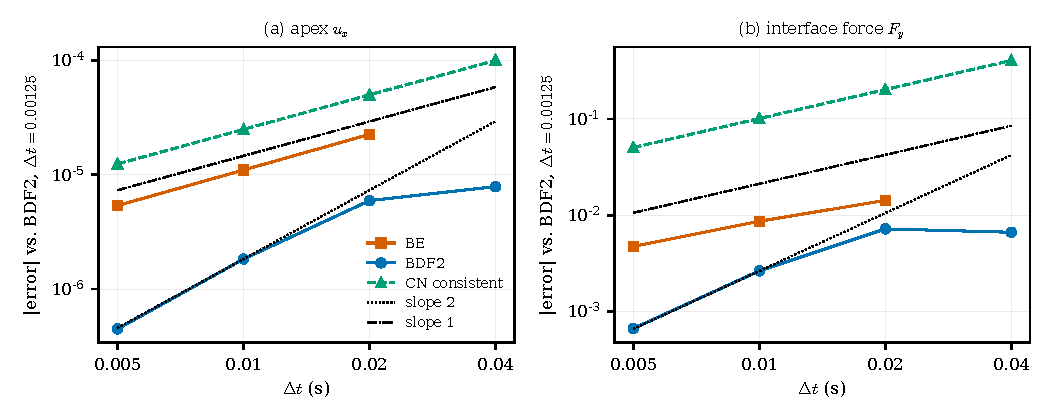
\includegraphics[width=\textwidth]{paper-data/fenicsx_blobintreacle/figures/fenicsx_blob_temporal}
\caption{blobInTreacle (FEniCSx, M2, $F=1$): error at $t=1$ against the independent BDF2 run with $\Delta t=0.00125$. BDF2 is second order only for $\Delta t\le0.01$; the two coarsest BDF2 levels ($0.04$, $0.02$) are pre-asymptotic. Source: \texttt{data/time\_values\_t1\_F1\_M2.csv}.}\label{fig:fx_temporal}
\end{figure}

\paragraph{What may and may not be said.}
\begin{itemize}
\item Steady states do not depend on the time step or the scheme (Section~\ref{sec:fx_steady}).
\item Backward Euler is first order for the apex $u_x$ ($p=1.04$); pointwise $u_y(1)$ is not accepted for any scheme.
\item BDF2 is second order for the apex $u_x$, apex $u_y$ and $F_y$ at $\Delta t\le0.01$ on this mesh, at this time, for M2: against the independent finer reference the pairwise orders are $2.03$, $2.32$ ($u_x$), $1.89$, $2.27$ ($u_y$), $1.99$, $2.29$ ($F_y$), within $0.05$ of the values a pure second-order error would give against a reference only a factor 2--8 finer.
$F_x$ fails the registered rule at one pair ($2.86>2.5$; every order is $\ge1.9$).
It is not shown for other times, other meshes, M1, or the interface velocity, and the coarse levels ($\Delta t=0.04$, $0.02$) are not asymptotic.
\item The consistent Crank--Nicolson scheme converges at first order for the displacement and the forces; with an added consistent weighting of the pressure geometry the displacement is second order while $F_x$, $F_y$ stay first order (an unresolved error source in the force evaluation), and a preregistered prediction that all three would reach order $\ge1.5$ was therefore only partly met.
Crank--Nicolson is not recommended: two earlier instabilities were implementation defects of the verifying code (a non-consistently weighted outlet and interface term), found and fixed after the fact.
BDF2 and the consistent Crank--Nicolson extrapolation reach the same time limit at $t=1$ ($F_x=7.60935$ and $7.60926\,\mathrm{N/m}$; $u_x$ $0.0575014$ and $0.0575011$), a cross-scheme check of the discrete time limit for $u_x$ and $F_x$.
\item A separate preregistered test on a different problem (an elastic wall in a channel) did \emph{not} confirm second order for the BDF2 interface velocity (finest-pair rates $1.56$ and $1.69$ outside $[1.7,2.5]$; displacement and fluid velocity were confirmed; Crank--Nicolson diverged at three levels).
The ``noise floor'' reading of that failure is an interpretation.
\item The error metric history: the primary metric was changed from the end-time error to an RMS over sample times after a first attempt failed, and the change was not preregistered; the RMS values are given in \texttt{data/time\_rms\_history\_t0\_1\_F1\_M2.csv} as additional information.
\item \textbf{No second-order temporal convergence is claimed for blobInTreacle.} The temporal-order statement of the main article concerns solids4foam; the solids4foam time-step series made here (apex $u_x(1)$ changes by at most $2.7\times10^{-4}$ between $\Delta t=0.04$ and $0.005$, by at most $9.2\times10^{-5}$ between $0.01$ and $0.005$) shows that the time error is small, but its order is not identified: successive differences are non-monotone at the $10^{-5}$ level in three of four series, at the level of the coupling tolerance and partition noise.
The solids4foam temporal order is neither confirmed nor refuted by this work.
No M1 time study exists beyond backward Euler (M1 Crank--Nicolson is unstable, M1 BDF2 is a single-mesh pilot), and backward Euler at $t=1$ for M1 has orders $0.46$--$0.62$, not asymptotic.
\end{itemize}

\paragraph{Pending: BDF2 transient spatial study at $t=1$.}
No FEniCSx spatial sequence exists at $t=1$, so no cross-code statement about the transient is made; the apparent equality of the FEniCSx $F=1$ BDF2 value ($0.057501$) with the solids4foam x2 value ($0.057496$) is a coincidence of different cell counts, not a comparison.
A BDF2 study at $\Delta t=0.005$ on $F=0.5$, $1$, $2$ (and $4$ if affordable), preregistered, is running.
\begin{table}[htbp]
\centering
\caption{PENDING: BDF2 transient spatial study at $t=1$, $\Delta t=0.005$, M2. To be filled from the run records; the $F=1$ row is the existing BDF2 run, all other entries are not results.}\label{tab:fx_pending}
\begin{tabular}{@{}lrrrrr@{}}
\toprule
Level & Cells & $u_x(1)$ & $u_y(1)$ & $F_x(1)$ & $F_y(1)$ \\
\midrule
$F=0.5$ & 150 & \pending{} & \pending{} & \pending{} & \pending{} \\
$F=1$ & 600 & 0.0575007 & $-0.0090796$ & 7.60937 & $-15.9557$ \\
$F=2$ & 2400 & \pending{} & \pending{} & \pending{} & \pending{} \\
$F=4$ & 9600 & \pending{} & \pending{} & \pending{} & \pending{} \\
Observed order, limit & & \pending{} & \pending{} & \pending{} & \pending{} \\
solids4foam M2 at equal $F$ & & \pending{} & \pending{} & \pending{} & \pending{} \\
\bottomrule
\end{tabular}
\end{table}
An interface-shape comparison at $t=1$ and $t=10$ with the preprint is likewise not part of this work.

%%%%%%%%%%%%%%%%%%%%%%%%%%%%%%%%%%%%%%%%%%%%%%%%%%%%%%%%%%%%%%%%%%
\section{Interface force and conservation}\label{sec:fx_force}
%%%%%%%%%%%%%%%%%%%%%%%%%%%%%%%%%%%%%%%%%%%%%%%%%%%%%%%%%%%%%%%%%%
Source: \texttt{data/force\_conservation\_evidence.csv}, \texttt{data/interface\_force\_bins\_M2\_F4.csv}.

\paragraph{Resultant transfer.}
Both codes transfer about $13$--$14\%$ less $x$-force to the solid under M2 than the fluid reports: the ratio of base reaction to fluid-reported force is $0.873$ at every FEniCSx level and $0.845$ to $0.869$ (x0.5 to x4) in solids4foam, and in solids4foam the written traction times the reference areas sums to $13.85$ against the fluid-reported $15.83\,\mathrm{N/m}$ at x1 (and $14.22$ against $16.27$ at x4), far above the $2$--$3\%$ accuracy of the force estimators used.
The FEniCSx base reaction balances the M2 force applied to the solid ($1.000$ to $1.002$).
At $t=1$ the M2 transfer delivers $3.4$--$3.5\%$ less interface power than the fluid supplies on the current surface (ratio $0.9653$ at x1, $0.9659$ at x2; exactly $1$ for E-AREA).
This is the strongest finding of the work; it is a property of the transferred force measure of a linear-geometry model, stated without a claim on solids4foam correctness.

\paragraph{Closure of the force balance.}
The weak-form balance closes algebraically: for the M1 solution at $F=1$, the fluid load (with the load on the two corner nodes counted once) and the support reactions sum to $4.5\times10^{-9}$ ($x$) and $1.4\times10^{-7}$ ($y$) of $|\bm F_\mathrm{fluid}|$, and the corner load, $(0.258,-0.605)\,\mathrm{N/m}$ ($1.6\%$ and $2.3\%$ of the total), is exactly the difference between the fluid-reported force and the support reaction.
That is an identity of the converged Galerkin residual (a sum of rows of the solved system): it checks convergence and bookkeeping, not the pointwise equilibrium of the traction.
For M2 the nodal figure is $0.03$--$0.09\%$.
An independent assembly of the pointwise stress over the interface and the base, however, closes only to $2.9\%$ ($F=1$) and $1.9\%$ ($F=2$) of $|\bm F_\mathrm{interface}|$, against a preregistered expectation of $10^{-6}$ that was \emph{not} met.
It is attributed to traction-recovery error at the floor--interface corners, decreasing with refinement, but only two levels exist, no order was determined, and the gap of a factor of $30$ to $100$ between the nodal and pointwise figures has not been explained beyond that.
The solids4foam side has the same limitation: the stress-based base reaction of the E-AREA runs misses the exactly known force by $1.8$--$2.5\%$, so no force-conservation check at the $1\%$ level exists there either.
Mass is conserved: $Q_\mathrm{in}=-Q_\mathrm{out}=1.125000$ at every level in the steady state, and the residual of $\mathrm{d}V/\mathrm{d}t+Q$ is a mesh-independent first-order time error.

\paragraph{Load distribution.}
At $F=4$ the per-bin M2 load on the solid of the coupled FEniCSx solution, the FEniCSx fluid solved on its own shape and on the solids4foam deformed shape, and the coupled solids4foam load agree to at most $0.014\,\mathrm{N}$ per $15^\circ$ bin in $F_x$ and $0.008\,\mathrm{N}$ in $F_y$; the FEniCSx load is insensitive to the interface shape ($0.013\%$) and to the interior mesh ($<0.001\%$).

%%%%%%%%%%%%%%%%%%%%%%%%%%%%%%%%%%%%%%%%%%%%%%%%%%%%%%%%%%%%%%%%%%
\section{Reproducibility}\label{sec:fx_repro}
%%%%%%%%%%%%%%%%%%%%%%%%%%%%%%%%%%%%%%%%%%%%%%%%%%%%%%%%%%%%%%%%%%
Every run is a Slurm job on one shared node with 2 to 8 MPI ranks, launched through a wrapper that fixes the MPICH/PETSc environment, and has a manifest with the code commit, the input and mesh hashes and the exit status of the driver (not of Slurm).
Preregistrations were written and hashed before the runs; the 26 hashes were re-verified by the reviewer.
A reproduction from fresh archives of the frozen commits gave the original $F=1$ M2 and M1 runs to $4\times10^{-15}$ relative at every step, and the $\Delta t=0.04$ steady values at $F=1$, $2$ to $4\times10^{-10}$.
The total campaign cost was $46.9$ CPU-hours for FEniCSx (including failed and cancelled jobs), of which the M1 mesh study took $3.2$ and the M2 backward-Euler family $13.2$ (including cancelled jobs).
Frozen commits, environment, mesh hashes, commands, data and scripts are in \texttt{paper-data/fenicsx\_blobintreacle/}; the data tables are regenerated from \texttt{data/steady\_levels.csv} by \texttt{scripts/analyze\_steady.py}, and the figures from the CSV files by \texttt{scripts/make\_figures.py}.
The raw solver histories and the code repository itself are not part of this pull request.

%%%%%%%%%%%%%%%%%%%%%%%%%%%%%%%%%%%%%%%%%%%%%%%%%%%%%%%%%%%%%%%%%%
\section{Limitations}\label{sec:fx_limits}
%%%%%%%%%%%%%%%%%%%%%%%%%%%%%%%%%%%%%%%%%%%%%%%%%%%%%%%%%%%%%%%%%%
\begin{itemize}
\item Same group, same agent family, same problem definition and mesh topology: a second implementation, not an independent verification (Section~\ref{sec:fx_scope}).
\item No temporal verification of the benchmark itself beyond the limited BDF2 result of Section~\ref{sec:fx_time}, no spatially converged transient, no interface-shape comparison, no M1 time study.
\item The model is not unique (M1 or M2), no statement is made on which one is correct, and the connection of M1 to the preprint rests on a coarse-mesh figure value.
\item Apex $u_y$ is not resolved below about $1\%$ between the two codes; the attribution of the gap rests partly on a reference chosen after the first comparison.
\item The pointwise force closure is $2$--$3\%$ at two levels; the x4 E-AREA level and a base-reaction test with an estimator of known accuracy are missing.
\item Observed orders of $u_x$ (1.4--1.5) and $F_y$ (0.9) are below two; the fluid mesh Jacobian degrades with refinement; geometry (chords against circle) contributes up to $0.15\%$ at $F=1$ and is not in the GCI; a few step-norm Newton acceptances occurred in transients.
\item Differences from the tutorial (outlet, mesh motion, convection, solid discretisation) are not isolated.
\item The solids4foam series is regenerated, with a $0.5\%$ inlet-flux error at x1.
\end{itemize}

%%%%%%%%%%%%%%%%%%%%%%%%%%%%%%%%%%%%%%%%%%%%%%%%%%%%%%%%%%%%%%%%%%
\section{Added value}\label{sec:fx_value}
%%%%%%%%%%%%%%%%%%%%%%%%%%%%%%%%%%%%%%%%%%%%%%%%%%%%%%%%%%%%%%%%%%
(i) The solids4foam steady state of the original model, previously supported by a coarse preprint figure and its own mesh sequence, is reproduced by a numerically different code to $0.05$--$0.2\%$ in $u_x$, force and pressure drop, with a Richardson limit and GCI for each.
(ii) The interface measure of the tutorial is identified from its source and its consequence is quantified: $13$--$14\%$ less $x$-force reaches the solid, $3.4\%$ less interface power at $t=1$, and a $7.5\%$ ($u_x$) and $16\%$ ($u_y$) model-form sensitivity that is stable under refinement.
(iii) The benchmark is shown to be a family of two models, which bears on how the C-weak reference of the main article should be read.
(iv) The limits of the temporal evidence are stated.
It does not provide an independent code, an established temporal order, or a decision between the two models.

\bibliography{bibliography}

\end{document}
